\documentclass[10pt]{article}

\usepackage[margin=0.75in]{geometry}
\usepackage{amsmath,amsthm,amssymb}
\usepackage{xcolor}
\usepackage{cancel}
\usepackage{graphicx}
\usepackage{changepage}
\usepackage{circuitikz}
\usepackage{minted}
\usepackage{pgfplots}
\usepackage{physics}
\usepackage{siunitx}
\usepackage[breakable]{tcolorbox}
\usepackage[inline]{enumitem}

\theoremstyle{definition}
\newtheorem{problem}{Problem}
\newtheorem{soln}{Solution}

\pgfplotsset{compat=newest}
\usetikzlibrary{lindenmayersystems}
\usetikzlibrary{arrows}

\definecolor{incolor}{HTML}{303F9F}
\definecolor{outcolor}{HTML}{D84315}
\definecolor{cellborder}{HTML}{CFCFCF}
\definecolor{cellbackground}{HTML}{F7F7F7}
\newcommand{\eq}{=}
\usetikzlibrary{positioning, fit, calc}
\pgfdeclarelayer{background}  
\pgfsetlayers{background,main}

\makeatletter
\newcommand{\boxspacing}{\kern\kvtcb@left@rule\kern\kvtcb@boxsep}
\makeatother
\newcommand{\prompt}[4]{
    \ttfamily\llap{{\color{#2}[#3]:\hspace{3pt}#4}}\vspace{-\baselineskip}
}

\newcommand{\thevenin}[2]{
  \begin{center}
    \begin{circuitikz} \draw
      (0,0) -- (2,0) to[battery1, l_=$V_{Th}\eq#1$] (2,2) 
      to[resistor, l_=$R_{Th}\eq#2$] (0,2)
      ;
      \draw [o-] (-.07,2.079);
      \draw [o-] (-.07,0.079);
    \end{circuitikz}
  \end{center}
}

\newcommand{\norton}[2]{
  \begin{center}
    \begin{circuitikz} \draw
      (0,0) -- (3,0) to[american current source, l_=$I_{N}\eq#1$] (3,2) -- (0,2) (2,0)
      to[resistor, l=$R_{N}\eq#2$] (2,2)
      ;
      \draw [o-] (-.07,2.079);
      \draw [o-] (-.07,0.079);
    \end{circuitikz}
  \end{center}
}

\newcommand{\highlight}[1]{\colorbox{yellow}{$\displaystyle #1$}}

\NewDocumentCommand{\evalat}{sO{\big}mm}{%
  \IfBooleanTF{#1}
   {\mleft. #3 \mright|_{#4}}
   {#3#2|_{#4}}%
}

\title{Math 2150: Assignment I}
\author{Jeremy Favro}
\date{\today}

\begin{document}

\maketitle
Note: I've kept $p$, $q$, and $r$ throughout my solutions and only substituted the actual numbers in at the end. This is because I find it easier,
especially when dealing with things that might cancel nicely, to deal with variables rather than the numbers they represent. In my case my 
student number is 0805980 so $p=9$, $q=5$, and $r=22$. Additionally, this document is the distilled form of my full process for solving all of these so there may at
points be some lacking detail as I've transcribed from my work on paper.
\\
% PROBLEM 1
\begin{problem}
Solve each of the following differential equations.
\begin{enumerate}[label=(\alph*)]
  \item $\displaystyle 2qy\sin(x)\cos(x)-py+2ry^2e^{xy^2}+\sec^2(qx)=\left(px+\cos(py)-q\sin^2(x)-4rxye^{xy^2}\right)\frac{dy}{dx}$
  \item $\displaystyle \frac{dy}{dx}=\frac{yx+px-qy-pq}{xy+ry-px-rp}$
\end{enumerate}
\begin{center}

\end{center}
\end{problem}
\begin{soln} ~\\
  \begin{enumerate}[label=(\alph*)]
    \item This is probably exact with $\displaystyle M=2qy\sin(x)\cos(x)-py+2ry^2e^{xy^2}+\sec^2(qx)$ and $N=-px-\cos(py)+q\sin^2(x)+4rxye^{xy^2}$.
          To proceed with solving it as an exact equation we need to check that $\displaystyle\frac{\partial M}{\partial y}=\frac{\partial N}{\partial x}$.
          $\displaystyle\frac{\partial M}{\partial y} =2q\sin(x)\cos(x)-p+4rye^{xy^2}+4rxy^3e^{xy^2}$ \\
          $\displaystyle\frac{\partial N}{\partial x} =-p+2q\sin(x)\cos(x)+4rye^{xy^2}+4rxy^3e^{xy^2}$ $\therefore \text{ this differential equation is exact.}$
          \begin{align*}
             & f(x,y)=C=\int M \,dx + h(y)                                                                       \\
             & =\int 2qy\sin(x)\cos(x)-py+2ry^2e^{xy^2}+\sec^2(qx) \,dx + h(y)                                   \\
             & =2qy\int \sin(x)\cos(x) \,dx - py\int \,dx + 2ry^2\int e^{xy^2} \,dx + \int\sec^2(qx) \,dx + h(y) \\
             & =qy\sin^2(x) - pyx + 2re^{xy^2} + \frac{1}{q}\tan(qx) + h(y)
          \end{align*}
          Then, $\displaystyle \frac{\partial f(x,y)}{\partial y}=N$
          \begin{align*}
             & \frac{\partial }{\partial y}\left[qy\sin^2(x) - pyx + 2re^{xy^2} + \frac{1}{q}\tan(qx) + h(y)\right]=N                                                     \\
             & \cancel{q\sin^2(x)} - \cancel{px} + \cancel{4rxye^{xy^2}} + \frac{dh(y)}{dy} =\cancel{-px}-\cos(py)+\cancel{q\sin^2(x)}+\cancel{4rxye^{xy^2} } \\
             & \frac{dh(y)}{dy} =-\cos(py) \implies h(y)=-\frac{1}{p}\sin(py)
          \end{align*}
          $\displaystyle\therefore f(x,y)=yx + 2re^{xy^2} + \frac{1}{q}\tan(qx) + \frac{1}{p}\sin(py)=5y\sin^2(x) - 9yx + 44e^{xy^2} + \frac{1}{5}\tan(5x) - \frac{1}{9}\sin(9y)=C$ where $C$ is some constant that can only be determined given
          initial conditions, which we do not have in this case. \newpage
    \item With some factoring this can be made more obviously seperable
          \begin{align*}
             & \frac{dy}{dx}=\frac{x(y+p)-q(y+p)}{y(x+r)-p(x+r)}   \\
             & \frac{dy}{dx}=\frac{(x-q)(y+p)}{(y-p)(x+r)}         \\
             & \frac{y-p}{y+p}dy=\frac{x-q}{x+r}dx               
          \end{align*}
          I'll solve both integrals seperately so I can better show what I'm doing. Starting with $y$:
          \begin{align*}
             & =\int \frac{y-p}{y+p}\,dy                                               \\
             & =\int \frac{y}{y+p}\,dy-p\int \frac{1}{y+p}\,dy                         \\
             & =\int \frac{y}{y+p}\,dy-p\ln(y+p)\rightsquigarrow u=y+p\implies du=dy   \\
             & =\int \frac{u-p}{u}\,dy-p\ln(y+p)                                       \\
             & =\int \frac{u}{u}\,du-p\int \frac{1}{u}\,du-p\ln(y+p)                   \\
             & =y+p-p\ln(y+p)-p\ln(y+p)+C                                              \\
             & =y+p(1-2\ln(y+p))+C                                                   
          \end{align*}
          Now for $x$:
          \begin{align*}
             & =\int \frac{x-q}{x+r}\,dy                                               \\
             & =\int \frac{x}{x+r}\,dy-q\int \frac{1}{x+r}\,dy                         \\
             & =\int \frac{x}{x+r}\,dy-q\ln(x+r)\rightsquigarrow u=x+r\implies du=dy   \\
             & =\int \frac{u-r}{u}\,du-q\ln(x+r)                                       \\
             & =\int \frac{u}{u}\,du-r\int \frac{1}{u}\,du-q\ln(x+r)                   \\
             & =x+r-r\ln(x+r)-q\ln(x+r)+C                                              \\
             & =x+r-(\ln(x+r))(r+q)+C                                                
          \end{align*}
          $\text{So the solution is } \displaystyle x+22-(\ln(x+22))(27)=y+9(1-2\ln(y+9))+C$
  \end{enumerate}
\end{soln}
\newpage
% PROBLEM 2
\begin{problem}
Solve each of the following initial value problems. Give your answers \textbf{explicitly} as a function of $x$.
\begin{enumerate}[label=(\alph*)]
  \item $\displaystyle \left(2pxy^2+2rxy\right)dx+\left(px^2y+rx^2+2py+2r\right)dy=0, \, y(1)=q$
  \item $\displaystyle (x+p)\frac{dy}{dx}+(qx+qp+1)y=3prx^2e^{px^3-qx}, \, y(0)=\frac{qr}{p}$
  \item $\displaystyle pyx\frac{dy}{dx}=py^2+x\sqrt{r^2x^2+y^2-q^2x^2}, \, y(1)=-q$
  \item $\displaystyle (p-1)(x+1)e^{rx}\frac{dy}{dx}+y^p=ry(1+x)e^{rx}, \, y(0)=-1$
\end{enumerate}
\begin{center}

\end{center}
\end{problem}
\begin{soln} ~\\
  \begin{enumerate}[label=(\alph*)]
    \item This looks exact, and almost is $\left(\displaystyle\frac{\partial M}{\partial y}=4pxy+2rx,\,\displaystyle\frac{\partial N}{\partial x}=2pxy+2rx\right)$. However, it's actually seperable
          \begin{align*}
             & 2xy\cancel{\left(py+r\right)}dx+\left[x^2\cancel{\left(py+r\right)}+2\cancel{\left(py+r\right)}\right]dy=0   \\
             & 2xydx+\left(x^2+2\right)dy=0                                                                                 \\
             & 2xydx=-\left(x^2+2\right)dy                                                                                  \\
             & -\frac{2x}{\left(x^2+2\right)}dx=\frac{1}{y}dy                                                               \\
             & -2\int \frac{x}{\left(x^2+2\right)}\, dx=\int\frac{1}{y}\,dy                                                 \\
             & -2\int \frac{x}{\left(x^2+2\right)}\, dx=\ln\left(y\right) \rightsquigarrow u=x^2+2\implies\frac{1}{2x}du=dx \\
             & -\int \frac{1}{u}\, du=\ln\left(y\right) + C                                                                 \\
             & -ln\left(x^2+2\right)=\ln\left(y\right) + C 
          \end{align*}
          Then we rearrange for $y$ and use the initial conditions to determine $C$
          \begin{align*}
             & -ln\left(x^2+2\right) + C=\ln\left(y\right) \\
             & \frac{C}{x^2+2}=y                           \\
             & y(1)=5=\frac{C}{x^2+2} \implies C=15
          \end{align*}
          So the solution is $y=\displaystyle\frac{15}{x^2+2}$
    \item This one is linear
          \begin{align*}
             & (x+p)\frac{dy}{dx}+(qx+qp+1)y=3prx^2e^{px^3-qx}                  \\
             & \frac{dy}{dx}+\frac{qx+qp+1}{x+p}y=\frac{3prx^2e^{px^3-qx}}{x+p} \\
          \end{align*}
          Our integrating factor is therefore 
          \begin{align*}
             & \displaystyle e^{\int \frac{qx+qp+1}{x+p}\, dx}                      \\
             & e^{q\int \frac{x+p}{x+p}\, dx + \int\frac{1}{x+p}\, dx}              \\
             & e^{qx+\ln\left(x+p\right)}=e^{qx}e^{\ln\left(x+p\right)}=(x+p)e^{qx}
          \end{align*}
          So,
          \begin{align*}
             & y(x+p)e^{qx}=\int (x+p)e^{qx}\frac{3prx^2e^{px^3-qx}}{x+p} \, dx                                            \\
             & y(x+p)e^{qx}=3pr\int x^2e^{px^3} \, dx                                                                      \\
             & y(x+p)e^{qx}=3pr\int x^2e^{px^3} \, dx \rightsquigarrow u=px^3\implies\frac{1}{3px^2}du=dx                  \\
             & y(x+p)e^{qx}=r\int e^{u} \, du                                                                              \\
             & y(x+p)e^{qx}=re^{px^3}+C                                                                                    \\
             & y=\frac{re^{px^3-qx}}{(x+p)}+\frac{C}{e^{qx}(x+p)}                                                          \\
             & y(0)=\frac{22e^{9(0)^3-5(0)}}{((0)+9)}+\frac{C}{e^{5(0)}((0)+9)} = \left(\frac{110}{9}\right)\implies C=88
          \end{align*}
          $\therefore y(x)=\displaystyle\frac{22e^{9x^3-5x}}{(x+9)}+\frac{88}{e^{5x}(x+9)}$
    \item This one is homogenous
          \begin{align*}
             & pyx\frac{dy}{dx}=py^2+x^2\sqrt{r^2+\frac{y^2}{x^2}-q^2}                                                 \\
             & pux^2(udx+xdu)=(pu^2x^2+x^2\sqrt{r^2+u^2-q^2})dx\rightsquigarrow u=\frac{y}{x}\implies dy=udx+xdu       \\
             & \cancel{pu^2x^2dx}+pux^3du=\cancel{pu^2x^2dx}+x^2\sqrt{r^2+u^2-q^2}dx                                   \\
             & pux^3du=x^2\sqrt{r^2+u^2-q^2}dx                                                                         \\
             & \frac{pu}{\sqrt{r^2+u^2-q^2}}du=\frac{1}{x}dx                                                           \\
             & p\int \frac{u}{\sqrt{r^2+u^2-q^2}} \, du=\ln(x)\rightsquigarrow s=r^2+u^2-q^2\implies \frac{1}{2u}ds=du \\
             & \frac{p}{2}\int \frac{1}{\sqrt{u}} \, du=\ln(x)                                                         \\
             & p\sqrt{r^2+u^2-q^2}=\ln(x)+C                                                                            \\
             & \frac{y^2}{x^2}-q^2=\frac{\ln^2(x)}{p^2}+C-r^2                                                          \\
             & y=\pm x\sqrt{\frac{\ln^2(x)}{p^2}+C+p^2-r^2+q^2}                                                        \\
             & y(1)=-1\sqrt{\frac{\ln^2(1)}{9^2}+C+9^2-22^2+5^2} = -5\implies C=403                                    \\
          \end{align*}
          $\therefore y(x)=-x\sqrt{\frac{\ln^2(x)}{81}+25}$
          \newpage
    \item My first thought with this one was that the $y^p$ probably means this one is a Bernoulli equation, which it is.
          \begin{align*}
             & (p-1)(x+1)e^{rx}\frac{dy}{dx}+y^p=ry(1+x)e^{rx}                                                                       \\
             & \frac{dy}{dx}+\frac{y^p}{(p-1)(x+1)e^{rx}}=\frac{ry}{p-1}                                                             \\
             & \frac{dy}{dx}-\frac{ry}{p-1}=-\frac{y^p}{(p-1)(x+1)e^{rx}} \rightsquigarrow\displaystyle \frac{dy}{dx}+P(x)y=Q(x)y^n
          \end{align*}
          Now we divide the whole thing by $y^p$ and substitute for $z=y^{1-p}$
          \begin{align*}
             & \frac{1}{\cancel{y^p}}\frac{\cancel{y^p}}{1-p}\frac{dz}{dx}-\frac{ry^{1-p}}{p-1}=-\frac{1}{(p-1)(x+1)e^{rx}} \rightsquigarrow z=y^{1-p}\implies \frac{y^p}{(1-p)}dz=dy \\
             & \frac{dz}{dx}-rz=-\frac{1}{(x+1)e^{rx}}
          \end{align*}
          Now that we've made the original equation linear we find the integrating factor
          \begin{align*}
             & \mu = e^{\int r\,dx}=e^{rx}
          \end{align*}
          So our linear ODE becomes
          \begin{align*}
             & rze^{rx}= \ln(x+1) + C                                                        \\
             & ry^{1-p}e^{rx}= \ln(x+1) + C                                                  \\
             & y^{1-p}= \frac{\frac{\ln(x+1)}{r} + C}{e^{rx}}                                \\
             & y= \pm\sqrt[1-p]{\frac{\frac{\ln(x+1)}{r} + C}{e^{rx}}}                       \\
             & y(0)= \pm\sqrt[1-9]{\frac{\frac{\ln(0+1)}{22} + C}{e^{22(0)}}}=-1\implies C=1 \\
          \end{align*}
          $\therefore y(x)=\displaystyle-\sqrt[-8]{\frac{\frac{\ln(x+1)}{22} + 1}{e^{22x}}}$
  \end{enumerate}
\end{soln}

\newpage
% PROBLEM 3
\begin{problem}
\textbf{SAGE}
\begin{enumerate}[label=(\alph*)]
  \item Consider the equation
        $$y^q\sin\left(y^p+x^q+x^r\right)=e^{\left(p-q\right)xy}-1$$
        \begin{enumerate}[label=\roman*.]
          \item Use the \textbf{diff} command to find the implicit derivative to obtain the differential equation for
                which this is an implicit solution.
                
          \item Plot the curve of the implicit solution on the rectangle using $-4 \leq x \leq 4$ and $-40 \leq y \leq 40$
                the command \textbf{implicit\_plot}.
          \item Describe the plot.
        \end{enumerate}
  \item Consider an indoor temperature $T_m$ that has oscillations that is driven by the outdoor temperature according to
        $$T_m=T_i=pe^{-\frac{1}{rq}t}\cos\left(\frac{\pi}{12}t\right)-re^{-\frac{1}{rq}t}\sin\left(\frac{\pi}{12}t\right)$$
        where $T_i = 70 + p-q$. Note that, that the oscillation has a 24 hour period and the cycle of the
        outdoor temperature repeats daily.
        \begin{enumerate}[label=\roman*.]
          \item Use the command \textbf{desolve} to find the general solution of the corresponding Newton's cooling
                equation.
          \item Apply the initial condition $T(0) = T_i + r$ to determine the particular solution.
          \item Apply the condition $T(1) = T_i + r-p$ to determine the constant $k$ in the Newton's cooling
                equation.
          \item Plot the particular solution the first 72 hours.
          \item Describe the plot
          \item Compute the average indoor temperature over the first 72 hours.
        \end{enumerate}
  \item Consider an indoor temperature $T_m$ that has oscillations that is driven by the outdoor temperature according to
        $$\frac{dy}{dx}=(y+p)^q\sin\left(qxy^p+1\right)\cos\left(pyx^q\right)e^{-\frac{1}{r}yx}$$
        \begin{enumerate}[label=\roman*.]
          \item Draw the associated direction field using \textbf{plot\_slope\_field}.
          \item Obtain the numerical solution of the differential equation subject to each of the initial
                conditions $y(0) = -4, -2, 0, 2, 4$ using \textbf{desolve\_rk4}. (ie. 5 IVP solution plots)
          \item Put the plots of each of the IVPs as well as the direction field plot on the same graph.
        \end{enumerate}
\end{enumerate}
\begin{center}

\end{center}
\end{problem}
\newpage
\begin{soln} ~\\
  \begin{enumerate}[label=(\alph*)]
    \item The graph looks garbled and messy but I believe that's how it's supposed to be.
          \begin{tcolorbox}[breakable, size=fbox, boxrule=1pt, pad at break*=1mm,colback=cellbackground, colframe=cellborder]
            \prompt{In}{incolor}{1}{\boxspacing}
            \begin{minted}[breaklines, autogobble]{sage}
clear_vars()
from IPython.core.interactiveshell import InteractiveShell
InteractiveShell.ast_node_interactivity = "all"
x = var('x')
y = var('y')

q = 5
p = 9
r = 22

x = var('x')
y = function('y')(x)
eq = y^q*sin(y^p+x^q+x^r)==e^((p-q)*x*y)-1
d = solve(diff(eq, x), diff(y,x))
show(d)

y = var('y')
eq = y^q*sin(y^p+x^q+x^r)==e^((p-q)*x*y)-1
implicit_plot(eq, (x,-4,4), (y,-40,40), aspect_ratio=0.1)
                      \end{minted}
          \end{tcolorbox}
          \begin{tcolorbox}[breakable, size=fbox, boxrule=.5pt, pad at break*=1mm, opacityfill=0]
            \prompt{Out}{outcolor}{1}{\boxspacing}
            $\displaystyle\left[\frac{\partial}{\partial x}y\left(x\right) = -\frac{{\left(22 \, x^{21} + 5 \, x^{4}\right)} \cos\left(x^{22} + y\left(x\right)^{9} + x^{5}\right) y\left(x\right)^{5} - 4 \, e^{\left(4 \, x y\left(x\right)\right)} y\left(x\right)}{9 \, \cos\left(x^{22} + y\left(x\right)^{9} + x^{5}\right) y\left(x\right)^{13} + 5 \, \sin\left(x^{22} + y\left(x\right)^{9} + x^{5}\right) y\left(x\right)^{4} - 4 \, x e^{\left(4 \, x y\left(x\right)\right)}}\right]$\\
            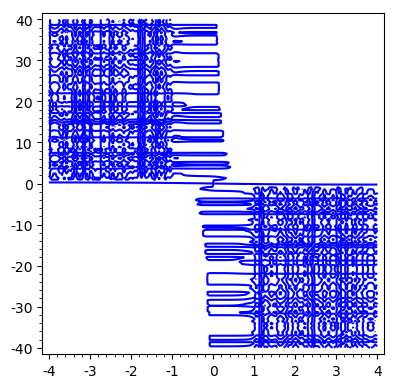
\includegraphics[scale=0.75]{G1.png}
            
          \end{tcolorbox}
          \newpage      
    \item The graph looks like a damped oscillation, which is what we'd expect as $T\to T_{avg}$ as $t\to\infty$
          \begin{tcolorbox}[breakable, size=fbox, boxrule=1pt, pad at break*=1mm,colback=cellbackground, colframe=cellborder]
            \prompt{In}{incolor}{1}{\boxspacing}
            \begin{minted}[breaklines, autogobble]{sage}
clear_vars()
from IPython.core.interactiveshell import InteractiveShell
from sage.symbolic.integration.integral import definite_integral
InteractiveShell.ast_node_interactivity = "all"
t, k = var('t, k')
T = function('T')(t)
dTdt = diff(T, t)

q = 5
p = 9
r = 22

T_i = 70 + p - q
A = T_i - p*e^(-1/(r*q)*t)*cos(pi/12*t)-r*e^(-1/(r*q)*t)*sin(pi/12*t)
show(A)

sol = desolve(dTdt==k*(T-A), T, ivar=t) # i
usol = desolve(dTdt==k*(T-A), T, ivar=t, ics=[0,T_i+r]) # ii
usolsub = (usol==T_i+r-p).subs(t==1)
kval = find_root(usolsub, -1, 0) # iii
plot(usol.subs(k==kval), 0, 72) # iv
tavg = definite_integral(usol.subs(k==kval), t, 0, 72)/72 #vi
show(N(tavg)) 
                      \end{minted}
          \end{tcolorbox}
          \begin{tcolorbox}[breakable, size=fbox, boxrule=.5pt, pad at break*=1mm, opacityfill=0]
            \prompt{Out}{outcolor}{1}{\boxspacing}
            $\displaystyle-9 \, \cos\left(\frac{1}{12} \, \pi t\right) e^{\left(-\frac{1}{110} \, t\right)} - 22 \, e^{\left(-\frac{1}{110} \, t\right)} \sin\left(\frac{1}{12} \, \pi t\right) + 74$\\
            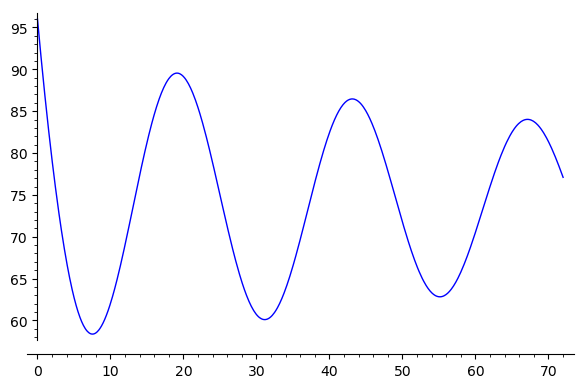
\includegraphics[scale=0.75]{G2.png} \\
            $74.2811410454468$
          \end{tcolorbox}
          \newpage
    \item ~
          \begin{tcolorbox}[breakable, size=fbox, boxrule=1pt, pad at break*=1mm,colback=cellbackground, colframe=cellborder]
            \prompt{In}{incolor}{1}{\boxspacing}
            \begin{minted}[breaklines, autogobble]{sage}
clear_vars()
x = var('x')
y = var('y')

# I changed these numbers because the actual values created a graph that did not demonstrate the slope field and function. This was done on the advice of Maya Peters.
q = 1
p = 4
r = 14

eqn = (y+p)^q*sin(q*x*y^p+1)*cos(p*y*x^q)*e^(-(1/r)*y*x)
sf = plot_slope_field(eqn, (x,-5,5), (y,-5,5))

p1=desolve_rk4(eqn, y, ics=[0,-4], output='plot', end_points=[-5,5], color="green")
p2=desolve_rk4(eqn, y, ics=[0,-2], output='plot', end_points=[-5,5], color="red")
p3=desolve_rk4(eqn, y, ics=[0,0], output='plot', end_points=[-5,5], color="blue")
p4=desolve_rk4(eqn, y, ics=[0,2], output='plot', end_points=[-5,5], color="orange")
p5=desolve_rk4(eqn, y, ics=[0,4], output='plot', end_points=[-5,5], color="purple")

show(p1+p2+p3+p4+p5+sf)
                      \end{minted}
          \end{tcolorbox}
          \begin{tcolorbox}[breakable, size=fbox, boxrule=.5pt, pad at break*=1mm, opacityfill=0]
            \prompt{Out}{outcolor}{1}{\boxspacing}
            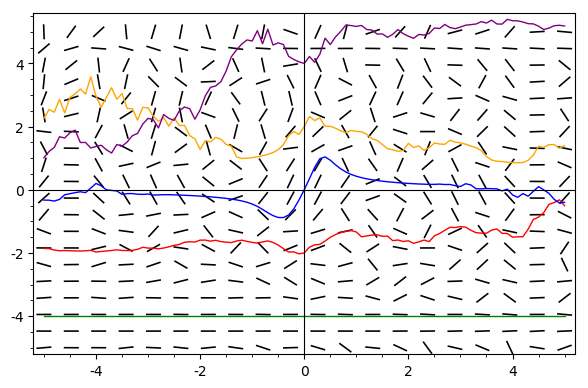
\includegraphics[scale=0.75]{G3.png} \\
          \end{tcolorbox}
  \end{enumerate}
\end{soln}
\end{document}